\chapter{Introduction}
The world wide web (WWW) got its popularity from its support for documents, images, videos, 3D graphics, and so on. The web is also excellent source of information that is made available through browsers.

A drawback of a basic web page is its limited behavior for dynamic content. This can be addressed by two types of programming extensions -  One is server-side programming languages and other is client-side programming languages \cite{LoginWeb}.

Server-side programming languages work on the server, which is situated across the network, and the browser has to keep sending information to the server to the process the input. There are lots of language choices available when it comes to programming on the server, such as Java, Python, JavaScript, and so on \cite{LoginWeb}. 

Client-side programming languages run in the browser, which helps to generate more dynamic content than simple web page can render \cite{Hickey:2004:SWP:1028174.971423}. But, there are very limited alternatives available when it comes to programming web pages in the browser such as JavaScript or Java.

As processing power in client-side machines is increasing, client-side programming is getting more popular among the software developer community. with that, feature list to be included in the specific preferences of client-side languages is growing. 

But, currently JavaScript is the ubiquitous language that runs in all browsers. JavaScript is used to enhance user interactivity within web pages and can change the way a web page looks and acts at any time, based on user input.

In this paper we are going to address building multi-language support for browsers, where more than one language can work in the browser at the same time and all these languages will interact together to render the web page. 


This paper is structured as follows :
Chapter 2 discusses the background research done in the field of multi-language environment; Chapter 3 discusses the Scheme environment and how it is implemented; Chapter 4 discusses the same details for Lua environement; Chapter 5 explains about how different environment interact with each other; Chapter 6 describes a sample how application can be built using Scheme, Lua and JavaScript working together in the same application; finally, chapter 7 concludes and presents opportunities for future work.

\section{Multi-language Browser Environment} 

Every programming language is different; some are more concise than others, while some are better in execution speed, or are closely related to underlying system and hardware. A multi-language environment can support interaction between software modules written in different programming languages.

Nowadays, most of non-trivial systems are not written in only one language.
Instead, many different languages are used; out of these are some general purpose programming languages like Ruby, Java, or JavaScript, but also some domain specific language (DSLs). A recent survey about open-source projects shows that the use of multi-language environment is rather universal. So, multi-language environment seems to be common, at least among open source groups \cite{Mayer2017}.

There are several benefits of having multi-language support in a browser, such as increase in productivity, benefit from multi-disciplinary client-side web pages development, and so on. Multi-language environment also supports different languages to work together, so that we can get best out of both worlds \cite{Matthews:2007:OSM:1190216.1190220}.


Currently, browser does not support multi-language environment. In this project, we built a multi-language environment in the browser for languages like Scheme \cite{Dybvig:2009:SPL:1618542}, Lua \cite{Ierusalimschy:2006:LRM:1215067}, and JavaScript. We enable support for these languages in the browser, by building our own parser and interpreter for a small subset of languages like Scheme, and Lua using JavaScript. These languages will interact with each other to render web page. We will see syntax and interaction of these languages in the upcoming sections. 


\subsection{Scheme Overview}

Scheme \cite{Dybvig:2009:SPL:1618542} is general purpose simple but powerful programming language.
 Scheme is widely used in computation research and education, it also used in industrial applications like user interface designs, web navigators to virtual reality engines \cite{Dybvig:1996:SPL:525334}. Scheme is formally standardized by IEEE \cite{schemeieee}.

Scheme program is block scoped. Variables and keywords in the Scheme program are lexically scoped. Occurence of the same identifier outside the block of code, refer to different identifier, otherwise reference is invalid. Blocks can also be nested in each other.

Scheme procedures are call-by-value. Procedures are also first object just like numbers, strings, and variable. Just like in other language, procedures can also be nested, and recursive. The same procedure can call itself. 

Let's take a look into small overview of Scheme, which will give us an idea of getting started with writing Scheme programs.

\subsubsection{Scheme Syntax}

This section give a small overview of Scheme as a language, to help us get some idea about Scheme.

Just like Lisp, Scheme programs are written as prefix expressions within parentheses for grouping. In Scheme name of the operation comes before its operand \cite{Krishnamurthi:1994:IS:197149.197166}.

Scheme program is combination of variables, objects, keywords, structured forms, comments, white spaces, and constant strings (numbers, vectors, strings, etc.)  \cite{SchemeLanguage}.


In C or most of languages, a procedure call to foo with arguments baz and bar looks is written like: 

\begin{lstlisting}
	foo(baz, bar);
\end{lstlisting}

But, in Scheme it is written as: 

\begin{lstlisting}
	(foo baz bar)
\end{lstlisting}

Variable can be defined using `define':

\begin{lstlisting} 
	(define myvariable 5)
\end{lstlisting}

This will tell the Scheme to allocate variable `myvariable' and assign value 5 to it. In the Scheme, variable value has to be defined always.

Procedure can also be created using `define' as shown:

\begin{lstlisting} 
	(define (two-times x)
		(* x x))
\end{lstlisting}


Above, code creates a procedure with name `two-times' with one argument. 

Just, like in any other languages if-else in Scheme can be implemented as follows:

\begin{lstlisting}
	(define (min a b)
		(if (< a b)
		 a	
		 b)
	)
\end{lstlisting}

It will create procedure called `min' with two arguments a and b. It will return minimum out of both variables by comparing variables in if statements. if a is less than b then return a, otherwise return b.

Scheme provides special procedure called lambda. Lambda does not give name to the procedure, it just returns the pointer to it.

We can use lambda in define statement, to assign it to variable as shown below:

\begin{lstlisting}
	(define double (lambda (x)
	   (+ x x )))
 
\end{lstlisting}


Here, we are creating procedure with one argument, and returning the pointer to it and we are storing that pointer into double variable using define.	 

\subsection{Lua Overview}

This section give an overview of Lua programming language \cite{Ierusalimschy:2006:LRM:1215067} and introduce the basic Lua concepts. 

Lua is designed to be a small, simple, fast, and portable language, which can be easily embedded into other applications \cite{spe96}. Lua is now popular among various type of application development such as, robotics, web development, image processing, distributed systems, extensible text editors, and more \cite{luaprojects}. Lua is one of the most popular scripting language for game development.

It is a procedural language with syntax like Pascal. It has control structures like (if , while, etc.). Procedure can have parameters, and local variables. Figure \ref{fig:luafactorial} below shows, implementation of factorial program in Lua.

\begin{figure}[h]
	\begin{lstlisting}
	function factorial (n)
	  local i = 1
	  local r = 1
	    while i <-n do 
	      r = r * i
	      i = i + 1
	    end
	  return r
 	end
	\end{lstlisting}
	\caption{Lua factorial example}
	\label{fig:luafactorial}
\end{figure}


\section{Goal}

Main goal of this project to provide richer variety of languages for client, by creating multi-language support for browser. It can be enabled by integrating client-side implementation of Scheme, Lua, with existing JavaScript. We will also dive deeper into questions like``How applications can benefit from it?" and ``How can we make multi-language environment easy to use?" by actually creating a demo application using multi-language environment in browser.

Another goal is to create browser plugin and client-side libraries for parsing and interpreting, Scheme and Lua using JavaScript. Also, implement language subset of these languages to interact with the document object model (DOM).

This project does not try to achieve most efficient solution to multi-language browser support. but we think that our solution will definitely help the software community by showing a way to how languages can interact.

\section{Approach}

There are variety of possible approaches to built multi-language support for the browser. In this project, we are going to focus on approach of using the browser plugin (Mozilla, Chrome) for proving multi-language support for the browser. 

\subsection{Browser Plugin } 

\begin{figure}[h]
	\begin{center}
		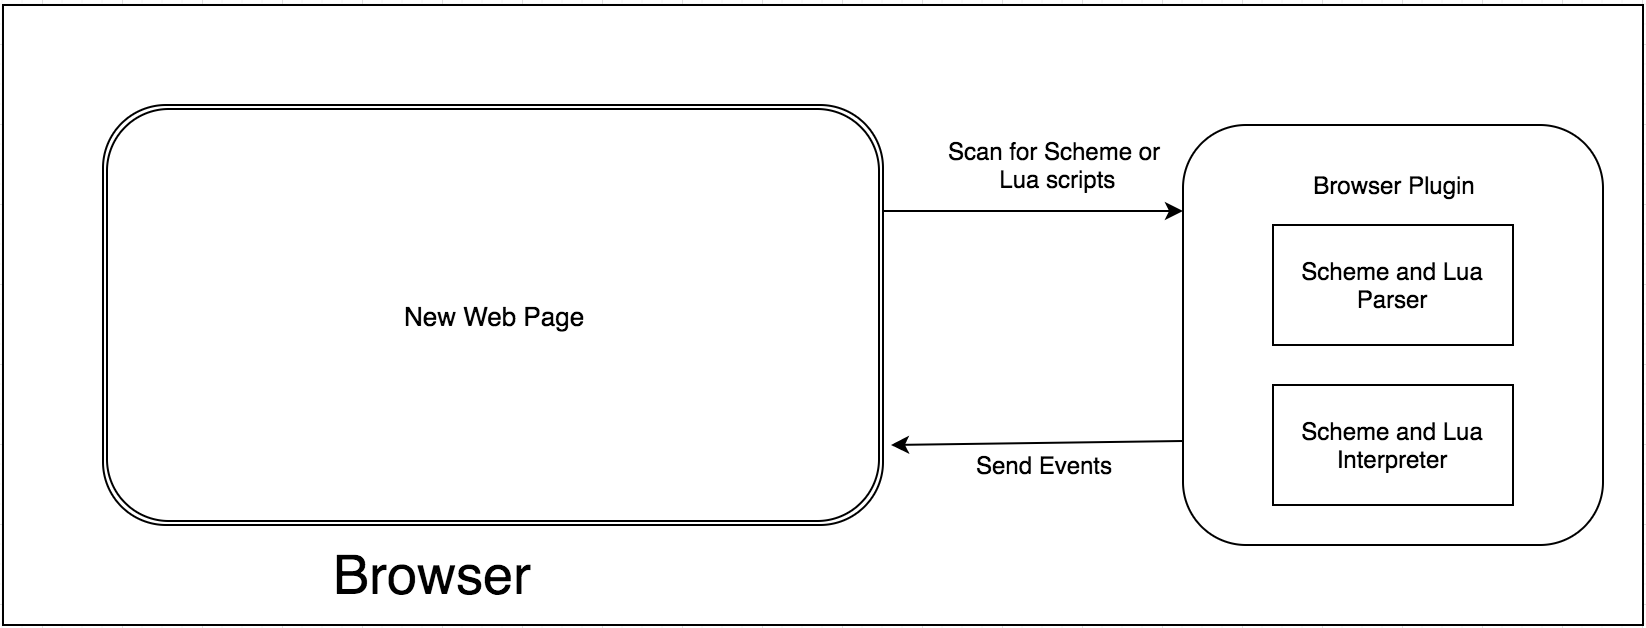
\includegraphics[width=\linewidth]{./images/browserPluginApproach.png}
	\end{center}
	\caption{Browser Plugin Approach : Architecture}
	\label{fig:pluginarchitecture}
\end{figure}

Multi-language support will be integrated into the web browsers (Mozilla, Chrome) using Mozilla and Chrome Plugin. The plugin will parse and then interpret any Scheme and Lua script on the page and will inject necessary events into the page again. As shown in Figure \ref{fig:pluginarchitecture}

Whenever, the new web page is loaded into the browser, plugin will scan the web page for any Scheme or Lua scripts on that page. Matching scripts will be parsed by the parser. Interpreter will interpret the parsed input into necessary DOM events. These events will be sent to the web page. 

All the interaction between languages is managed by browser plugin. Advantage of having this approach is, programmer does not have to worry about adding all the multi-language supporting libraries into the web page. Disadvantages of having this approach is, plugin needs to be installed in the browser and some browsers are not yet supported by the plugin. Also, plugin need a permission to read scripts from the web page. We overcome this disadvantage, by exposing Scheme and libraries, which can be included in the web page directly.

\subsubsection{JS Library}

\begin{figure}[h]
	\begin{center}
		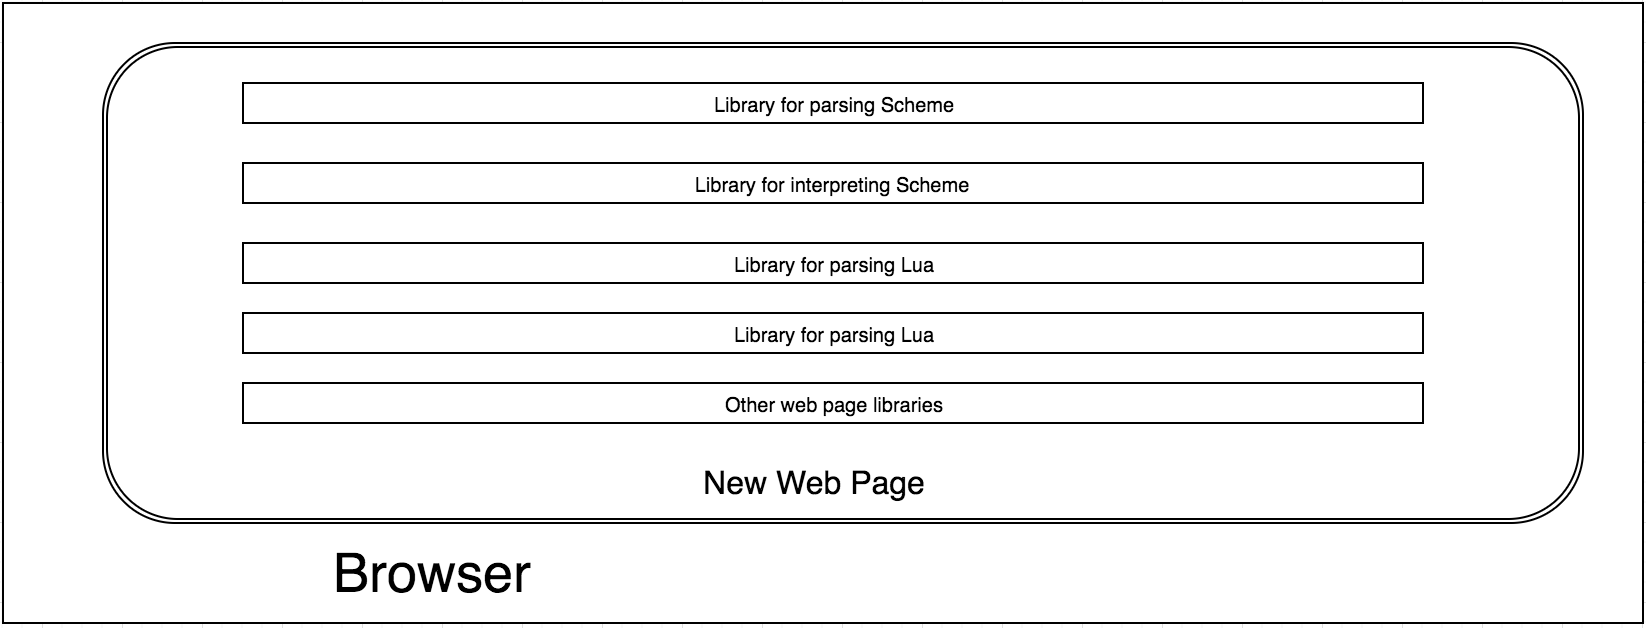
\includegraphics[width=\linewidth]{./images/JSLibraryApproach.png}
	\end{center}
	\caption{JS Library Approach : Architecture}
	\label{fig:jslibraryarchitecture}
\end{figure}

If plugin is not available in the browser, multi-language support can be achieved by including supported libraries in the web page itself. Developer can include multi-language supporting libraries in the web page. After all libraries are loaded, browser will interpret different languages on the web page and help to achieve necessary interaction between these different languages. Libraries can be included in browser as shown in Figure \ref{fig:jslibraryarchitecture}.
\section{Challenges}

There are many challenges while building the multi-language support for any application. For building multi-language support for browser, these are some of the challenges that we came across.

\subsection{Different APIs for DOM}

To render web pages on the browser, language has to work with browser's DOM APIs. Every language has its own syntax for interacting with DOM APIs. 

Currently, there is no implementation of Scheme, and Lua in the browser. For this project, we created our own subset of Scheme and Lua, which works with browser's DOM APIs, and JavaScript.  We created our own parser and interpreter for these languages in browser, as discussed in Section \ref{scheme} and Section \ref{lua}

\subsection{Interaction between different languages}

Every developer use different tools and technologies, each of which might have different types, features, and purpose. Each language has different way of representing types, data, object, and etc. So, it is historically very difficult to ensure language interoperability. For this project, we created basic utilities for language interaction to happen smoothly, as discussed in Section \ref{interaction}..

\section{Results}

The contributions of this project;

1) Parser and Interpreter libraries for Scheme and Lua with support for DOM and interaction with JavaScript.

2) Browser plugin for Chrome and Firefox, which can execute Scheme and Lua scripts from any page opened in the browser.

3) A proof of concept Application, built using JavaScript, Scheme, and Lua working together.
